\chapter{Funcionamiento interno de Tremor}\label{annex:tremor}

\section{Arquitectura}

Antes de comenzar a modificar el código existente en Tremor, era importante
conocer cómo funciona para evitar perder el tiempo. Tremor se basa en el modelo
actor. Citando Wikipedia:

TODO: puedo citar Wikipedia?

% ORIGINAL:
% ``[The actor model treats the] actor as the universal primitive of concurrent
% computation. In response to a message it receives, an actor can: make local
% decisions, create more actors, send more messages, and determine how to
% respond to the next message received. Actors may modify their own private
% state, but can only affect each other indirectly through messaging (removing
% the need for lock-based synchronization).''

``[El modelo actor trata al] actor como el componente universal de computación
concurrente. En respuesta a un mensaje que recibe, un actor puede: tomar
decisiones locales, crear más actores, enviar más mensajes y determinar cómo
responder al siguiente mensaje recibido. Los actores pueden modificar su propio
estado privado, pero solo pueden afectarse entre sí indirectamente a través de
mensajería (eliminando la necesidad de sincronización con
\emph{locks}).''~\cite{wikiactor}

No usa un lenguaje (e.g., Erlang) o framework (e.g., \cratelink{bastion}, quizá
en el futuro) que siga estrictamente este modelo, pero re-implementa los mismos
patrones frecuentemente de forma manual. Tremor se basa en \emph{programación
asíncrona}, es decir, que en vez de hilos trabaja con \emph{tareas}, un concepto
de nivel más alto y especializado para entrada/salida. De la documentación de
\cratelink{async-std}, la runtime asíncrona que usa Tremor:

% ORIGINAL:
% ``An executing asynchronous Rust program consists of a collection of native OS
% threads, on top of which multiple stackless coroutines are multiplexed. We
% refer to these as “tasks”. Tasks can be named, and provide some built-in
% support for synchronization.''

``La ejecución de un programa asíncrono en Rust consiste en una recopilación de
hilos nativos del Sistema Operativo, sobre los cuales múltiples corutinas no
apilables (\emph{stackless}) son multiplexadas. Nos referimos a ellas como
``tareas''. Las tareas pueden tener nombre e incluir soporte para
sincronización.''~\cite{asyncstd_task}

Podríamos resumir su arquitectura con la frase ``Tremor se basa en actores
corriendo en tareas diferentes, que se comunican asíncronamente con canales''.

\section{Detalles de implementación}

El actor principal se llama \rust{World}. Contiene el estado del programa, como
los artefactos disponibles (\emph{repositorios}) y los que se están ejecutando
(\emph{registros}) y se usa para inicializar y controlar el programa.

Los \emph{managers} o \emph{gestores} son simplemente actores en el sistema que
envuelven una funcionalidad. Ayudan a desacoplar la comunicación y la
implementación de la funcionalidad interna. De esta forma, se puede eliminar
código repetitivo al inicializar los componentes, así como la creación de
canales de comunicación o el lanzamiento del componente en una tarea nueva.
Generalmente, hay un gestor por cada tipo de artefacto para facilitar su
inicialización y también uno por cada instancia que se esté ejecutando, para
controlar su comunicación.

Notar que la inicialización de los conectores ocurre en dos pasos. Primero se
\emph{registran}, es decir, se indica su disponibilidad para cargarlo
(añadiéndolo al repositorio). Posteriormente, no se ejecutará hasta conectarse
con otro artefacto con \rust{launch_binding}, lo cual lo movería del repositorio
al registro, junto al resto de artefactos ejecutándose.

\begin{figure}[h]
    \centering
    \begin{minted}{rust}
pub trait Connector {
    /// Crea la parte "source" del conector, si es aplicable.
    async fn create_source(
        &mut self,
        _source_context: SourceContext,
        _builder: source::SourceManagerBuilder,
    ) -> Result<Option<source::SourceAddr>> {
        Ok(None)
    }

    /// Crea la parte "sink" del conector, si es aplicable.
    async fn create_sink(
        &mut self,
        _sink_context: SinkContext,
        _builder: sink::SinkManagerBuilder,
    ) -> Result<Option<sink::SinkAddr>> {
        Ok(None)
    }

    /// Intenta conectarse con el mundo exterior. Por ejemplo, inicia la
    /// conexión con una base de datos.
    async fn connect(
        &mut self,
        _c: &ConnectorContext,
        _attempt: &Attempt
    ) -> Result<bool> {
        Ok(true)
    }

    /// Llamado una vez cuando el conector inicia.
    async fn on_start(&mut self, _c: &ConnectorContext) -> Result<()> {
        Ok(())
    }
    /// Llamado cuando el conector pausa.
    async fn on_pause(&mut self, _c: &ConnectorContext) -> Result<()> {
        Ok(())
    }
    /// Llamado cuando el conector continúa.
    async fn on_resume(&mut self, _c: &ConnectorContext) -> Result<()> {
        Ok(())
    }
    /// Llamado ante un evento de "drain", que se asegura de que no
    /// lleguen más eventos a este conector.
    async fn on_drain(&mut self, _c: &ConnectorContext) -> Result<()> {
        Ok(())
    }
    /// Llamado cuando el conector para.
    async fn on_stop(&mut self, _c: &ConnectorContext) -> Result<()> {
        Ok(())
    }
}
    \end{minted}
    \caption{Simplificación del \trait \rust{Connector}}%
    \label{fig:tremor_connector_trait}
\end{figure}

\subsection{Registro}

La Figura~\ref{fig:tremor_registering} detalla todos los pasos seguidos en el
código. Primero han de inicializarse los gestores, y después registrar los
artefactos. Actualmente, esta parte se realiza de forma estática con
\rust{register_builtin_types}, pero después de implementar el PDK, debería ser
dinámicamente. Tremor buscaría automáticamente plugins en sus directorios
configurados e intentaría registrar todos los que encuentre. En una futura
versión, el usuario podría solicitar manualmente el cargado de un plugin nuevo
mientras se está ejecutando Tremor.

\begin{figure}
    \centering
    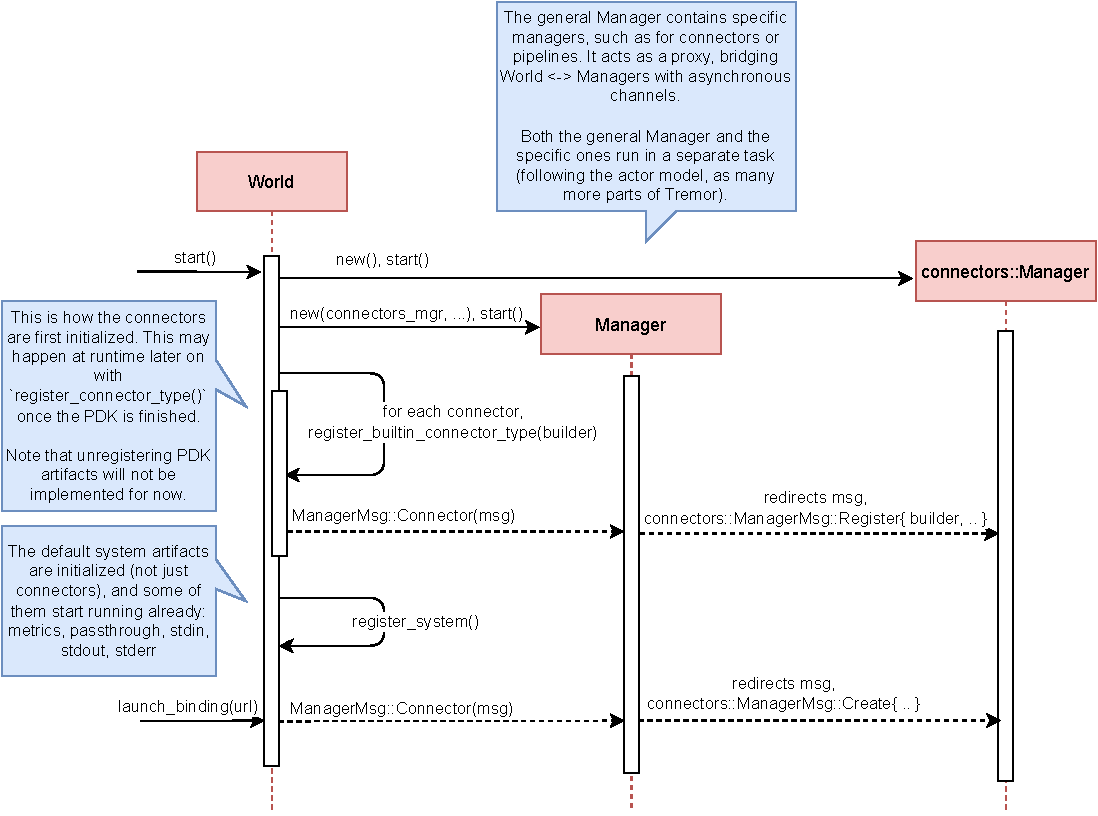
\includegraphics[width=\textwidth]{./Imagenes/registering.pdf}
    \caption{Registro de un conector en el programa}%
    \label{fig:tremor_registering}
\end{figure}

\subsection{Inicialización}

Ya que es un proceso en múltiples pasos (en la implementación es más complicado
que registro + creación), la primera parte provee las herramientas para
inicializar el conector (el \emph{builder}). Cuando el conector necesite
comenzar a ejecutarse porque se haya añadido a una \pipeline, el \builder ayuda
a construir y configurarlo de forma genérica. Finalmente, se añade a una tarea
propia para que se pueda comunicar con otras partes de Tremor. El gestor
\rust{connectors::Manager} contiene todos los conectores ejecutándose en Tremor,
como se muestra en la Figura~\ref{fig:tremor_initializing}.

\begin{figure}
    \centering
    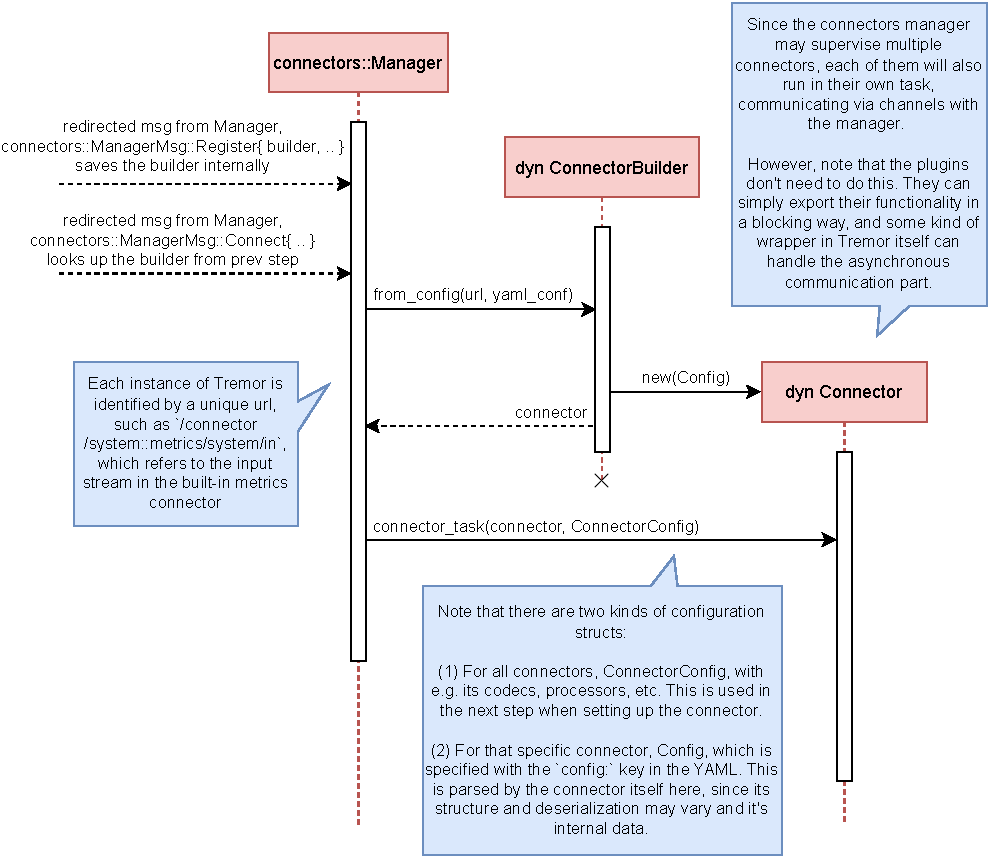
\includegraphics[width=\textwidth]{./Imagenes/initializing.pdf}
    \caption{Inicialización de un conector en el programa}%
    \label{fig:tremor_initializing}
\end{figure}

\subsection{Configuración}

Una vez haya un conector corriendo, la Figura \ref{fig:tremor_setting_up}
visualiza cómo se divide en una parte \sink y otra \source. Estas son
opcionales, pero no exclusivas, así que se puede tener cualquiera de las dos o
ambas. De forma similar, un \builder se usa para inicializar las partes y a
continuación inicia una nueva tarea para ellos.

\begin{figure}
    \centering
    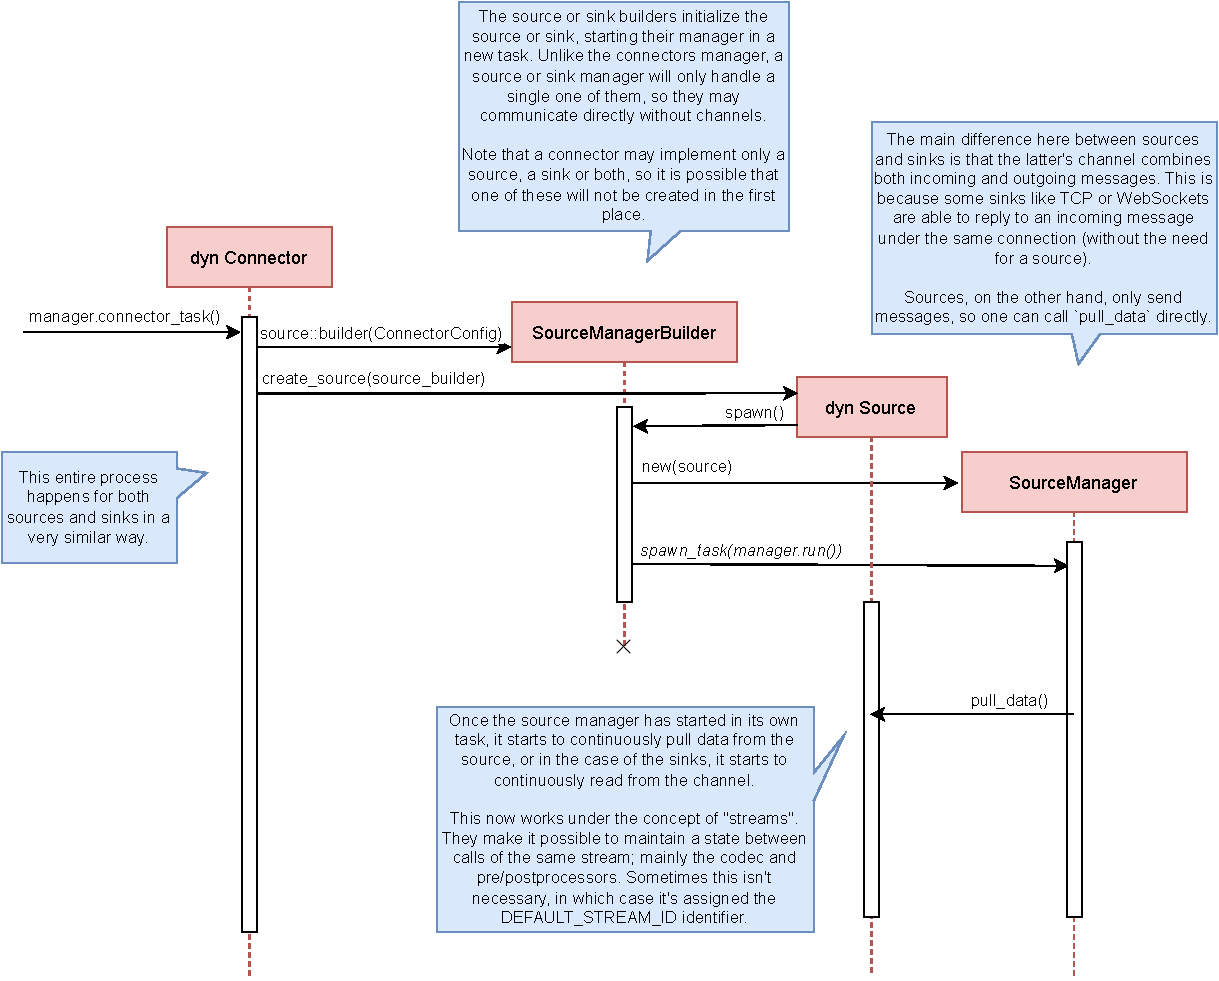
\includegraphics[width=\textwidth]{./Imagenes/setting-up.pdf}
    \caption{Configuración de un conector en el programa}%
    \label{fig:tremor_setting_up}
\end{figure}

También se crea un gestor por cada instancia de \sink o \source, que se
encargará de la comunicación con otros actores. De esta forma, sus interfaces
pueden mantenerse lo más simple posible. Esos gestores recibirán peticiones de
conexión de la \pipeline y posteriormente leerán o enviarán eventos en ella.

La diferencia principal entre \sources y \sinks a nivel de implementación es que
este último también puede responder a mensajes usando la misma conexión. Esto es
útil para notificar que el paquete ha llegado (\rust{Ack}) o que algo ha fallado
(\rust{Fail} para un evento específico, \rust{CircuitBreaker} para dejar de
recibir datos por completo).

Los códecs y preprocesadores se involucran aquí tanto para los \sources como
para los \sinks. En la parte de \source, los datos son transformados a través de
una cadena de preprocesadores y posteriormente se aplica un códec. Para los
\sinks, se sigue el proceso inverso: los datos se codifican primero a bytes con
el códec, y posteriormente una serie de postprocesadores se aplican a los datos
binarios.

\subsection{Notas adicionales}

Algunos conectores se basan en \emph{flujos}. Son equivalentes a los flujos de
TCP, que ayudan a agrupar mensajes para evitar mezclarlos. Se inician y
finalizan mediante mensajes, y el gestor se guarda el estado del flujo en un
campo llamado \rust{states} (ya que, por ejemplo, algunos preprocesadores puedan
querer guardar un estado). Si un conector no necesita flujos, como
\rust{metronome} (que únicamente envía eventos periódicamente), puede
especificar su identificador de flujo como \rust{DEFAULT_STREAM_ID} siempre.

Tras implementar la interfaz de los conectores para el sistema de plugins,
los primeros conectores a desarrollar deberían ser:

\begin{itemize}
    \item \emph{Blackhole}, usado para medir el rendimiento. Realiza mediciones
        de tiempos de final a final para cada evento pasando por la \pipeline, y
        al final guarda un histograma HDR (\emph{High Dynamic Range}).

    \item \emph{Blaster}, usado para repetir una serie de eventos de un archivo,
        que es especialmente útil para pruebas de rendimiento.

\end{itemize}

Ambos son relativamente simples y serán de gran ayuda para medir el efecto de
los cambios sobre el rendimiento. De todos modos, el equipo de Tremor insistía
que lo más importante primero es que funcione, y después me podría preocupar
sobre eficiencia.
